\documentclass[12pt]{article}

% Packages for Advanced Formatting
\usepackage{geometry}
\geometry{margin=1in}
\usepackage{amsmath}
\usepackage{amssymb}
\usepackage{tikz}
\usetikzlibrary{calc}
\usepackage{xcolor}
\usepackage{graphicx}
\graphicspath{{.}}
\usepackage{booktabs}
\usepackage{tabularx}
\usepackage{array}
\usepackage{listings}
\usepackage{setspace}
\usepackage{titlesec}
\usepackage{ragged2e}
\usepackage{indentfirst}
\usepackage{csquotes}
\usepackage[hidelinks]{hyperref}
\usepackage[style=apa, backend=biber]{biblatex}
\addbibresource{references.bib}

% Color Definitions
\definecolor{dlsugreen}{HTML}{00703C}

% R Code Listings Configuration
\lstset{
  language=R,
  basicstyle=\small\ttfamily,
  breaklines=true,
  keepspaces=true,
  columns=flexible,
  showstringspaces=false,
  keywordstyle=\color{blue},
  commentstyle=\color{dlsugreen},
  stringstyle=\color{purple},
  backgroundcolor=\color{gray!5},
  frame=single,
  framerule=0pt,
  xleftmargin=10pt,
  xrightmargin=10pt,
  aboveskip=15pt,
  belowskip=15pt
}

% APA 7th Edition: Headings & Indents
\titleformat{\section}{\normalfont\Large\bfseries\centering}{\thesection}{1em}{}
\titleformat{\subsection}{\normalfont\large\bfseries}{\thesubsection}{1em}{}
\titlespacing*{\section}{0pt}{12pt}{6pt}
\titlespacing*{\subsection}{0pt}{12pt}{6pt}
\setlength{\bibhang}{0.5in}

\begin{document}
\doublespacing
\RaggedRight
\setlength{\parindent}{0.5in}

\begin{titlepage}
    \centering

    % Top Logo and Name (Inline)
    \vspace*{0.5cm}
    \begin{tabular}{c@{\quad}l}
        \raisebox{-2.0ex}{
\includegraphics[height=3.5em]{dlsu_logo.png}} & 
        \huge \textbf{\color{dlsugreen} De La Salle University}
    \end{tabular}
    
    \vfill

    % Central Seal
    
\includegraphics[width=0.25\textwidth]{dlsu_logo.png} \\

    \vfill

    % Project Title
    {\LARGE \textbf{Hybrid Econometric and Machine Learning Modeling of Philippine Stock Returns}} \\
    \vspace{0.5cm}
    {\large A Multi-Horizon Predictive Analysis of Bank of the Philippine Islands (BPI) on the Philippine Stock Exchange} \\
    \vspace{1.5cm}

    \begin{minipage}{0.8\textwidth}
        \centering
        {\normalsize Final Project Case Study \\ {} Presented to \\ {} \textbf{Professor Bobby Baylon Jr.} \\ {} Department of Finance}
    \end{minipage}

    \vfill

    \begin{minipage}{0.8\textwidth}
        \centering
        {\normalsize in partial fulfillment of the requirements for the course \\ {} \textbf{FINLYTS}}
    \end{minipage}

    \vfill

    {\normalsize By:} \\
    \vspace{0.5cm}
    {\normalsize 
    ABRIL, Jehan \\
    {} GO, Keira Ley Arcala \\
    {} SISON, Aaron Joshua Estacio \\
    {} VALENCIA, Carlos Martin Belangel}

    \vfill

    {\normalsize \today}
\end{titlepage}

\newpage
\tableofcontents
\newpage

% ABSTRACT
\begin{abstract}
    % TODO: Write last. 150-200 words.
    % Cover: objective, data, models used, key finding, horizon comparison result.
\end{abstract}

\newpage

% SECTION 1: INTRODUCTION
\section{Introduction}
\label{sec:intro}
% ASSIGNED TO: Jehan

\textbf{\color{red}[TODO: Jehan --- Insert additional historical or qualitative context for the Philippine economy here to expand the introduction to the required 1.5--2 pages.]}

Forecasting equity returns in frontier markets is a monument to statistical futility under static linear assumptions. 
 The Philippine Stock Exchange (PSE) exhibits adaptive inefficiency driven by shifting volatility regimes \parencite{ahmed2022adaptive}. This study targets the banking sector through Bank of the Philippine Islands (BPI) and BDO Unibank (BDO). These institutions function as the primary transmission mechanism for domestic monetary policy. Their combined market capitalization ensures high liquidity and systemic relevance. They represent the most robust proxy for Philippine macroeconomic health.

The choice of the banking industry is a monument to systemic risk concentration. Financial services dominate the PSEi weighting. BPI and BDO are the undisputed leaders in domestic credit intermediation. These entities generate the largest share of systemic risk in the Philippine economy \parencite{godoy2025measuring}. Investors use these tickers to express a view on the broader Philippine growth story. Their price action reflects both retail sentiment and institutional capital flows. Modeling their returns provides a diagnostic view of the national economy.

Local equity valuations are deterministic outputs of global liquidity conditions. The U.S. 10-Year Treasury Yield serves as the "global gravity" for all risky assets. Rising yields in developed markets trigger capital outflows from frontier regions. The USD/PHP exchange rate captures this currency-channel risk. It also tracks the impact of remittance-driven liquidity on domestic consumption. These variables are the non-negotiable anchors of any predictive framework.

This research evaluates the predictive efficacy of hybrid modeling architectures. Traditional OLS benchmarks fail to capture high-dimensional non-linear interactions. We deploy four machine learning algorithms to bridge this analytical gap. These include Random Forest, Support Vector Machines, XGBoost, and Artificial Neural Networks. The primary objective is to forecast returns across one-day, three-day, and five-day horizons. We hypothesize that machine learning architectures will definitively outperform linear benchmarks. They isolate regime-specific momentum patterns that linear models ignore.


% SECTION 2: LITERATURE REVIEW
\section{Literature Review}
\label{sec:litreview}

\subsection{The Adaptive Market Hypothesis in Frontier Markets}
Unconditional weak-form efficiency systematically fails to describe equity pricing in frontier markets. Empirical evidence from six ASEAN economies reveals that market inefficiency predictably spikes during systemic macroeconomic crises \parencite{huynh2025composite}. Consequently, the Adaptive Market Hypothesis provides a more precise framework for understanding cyclical predictability driven by shifting volatility regimes \parencite{ahmed2022adaptive}. This adaptive inefficiency manifests within the Philippine Stock Exchange (PSE) as distinct, exploitable patterns of momentum and mean reversion. Dynamic factor modeling of the PSE confirms that latent macroeconomic trends persistently drive predictable out-of-sample price movements \parencite{lim2026dynamic}. Frontier market predictability ultimately stems from delayed institutional information processing and reactive retail liquidity dynamics.

\subsection{Econometric Limitations and Machine Learning Efficacy}
Ordinary Least Squares (OLS) regressions structurally fail to map high-dimensional, multicollinear financial data. A canonical comparative analysis demonstrates that tree-based ensembles and neural networks definitively outperform traditional linear models \parencite{gu2020empirical}. These advanced architectures optimize predictive accuracy by computationally capturing deep non-linear interactions between momentum, localized liquidity, and historical volatility. Tree-based ensembles actively mitigate the curse of dimensionality without imposing rigid, pre-specified additive constraints. An equal-weighted ensemble of these algorithms successfully isolates highly profitable out-of-sample statistical arbitrage signals \parencite{krauss2017deep}. Machine learning models thus replace manual feature engineering with automated, data-driven mathematical abstraction.

\subsection{Sequential Memory and the Ensemble Approach}
Deep learning architectures are uniquely required to extract chronological sequence dependencies from financial time series. Long Short-Term Memory (LSTM) networks consistently outperform memory-free classification models by explicitly retaining long-term structural dependencies \parencite{fischer2018deep}. These memory gates allow LSTMs to isolate optimal trading signals driven by high localized volatility and short-term reversal profiles. However, the application of highly parameterized neural networks must contend with the No Free Lunch theorem of mathematical optimization. Machine learning architectures capturing deep non-linear patterns frequently fail to translate statistical predictability into profitable trading strategies \parencite{bustos2025machine}. Therefore, hybrid ensemble methodologies remain essential to hedge against shifting macroeconomic distributions and algorithmic vulnerabilities \parencite{waldow2021machine}.

\subsection{Macroeconomic Drivers of Philippine Banking Equities}
Philippine banking equities function as deterministic outputs of highly specific, systemic macroeconomic variables. The domestic banking sector consistently generates the absolute largest share of aggregate systemic risk within the Philippine economy \parencite{godoy2025measuring}. This extreme vulnerability is directly driven by exogenous macroeconomic shocks to domestic output, policy rates, and currency valuations. Furthermore, domestic currency depreciation substantially alters economic liquidity and fundamentally impacts corporate balance sheet risk profiles \parencite{tancangco2024effects}. For systemically critical entities like BDO and BPI, valuations remain highly sensitive to net open foreign exchange positions. Any robust predictive model must mathematically capture these non-linear macroeconomic transmission mechanisms alongside traditional pricing indicators.

\subsection{Multi-Horizon Predictability and Signal Decay}
The mathematical forecasting horizon fundamentally dictates the underlying signal-to-noise ratio of equity return predictions. One-day forecasts are overwhelmed by microstructure noise, restricting high-frequency statistical arbitrage strictly to transient mean reversion. Conversely, extending forecasts to five-day horizons successfully smooths execution noise to expose persistent, structural macroeconomic trends. This extension introduces the mathematical phenomenon of horizon decay, severely degrading predictive accuracy due to compounding exogenous uncertainty. Consequently, hybrid predictive frameworks must deploy multi-horizon architectures to simultaneously capture short-term reversals and medium-term momentum channels. Maximizing risk-adjusted returns requires precise temporal alignment between the chosen algorithmic architecture and the specific prediction target.

% SECTION 3: DATA AND FEATURE ENGINEERING
\section{Data and Feature Engineering}
\label{sec:data}
% ASSIGNED TO: Person 1 (data sourcing) + Person 2 (writing)
% Approx. length: 3 to 4 pages plus tables

\subsection{Data Sources and Sample Period}

The analysis draws on four daily price series retrieved from Investing.com, spanning January 2, 2019 to April 1, 2026---a final sample of 1,853 observations covering roughly 7.25 years of market activity. These series, detailed in Table \ref{tab:data_sources}, encompass the target equity, a sector-specific competitor, a broad market benchmark, and a macroeconomic proxy for currency-channel risk.

\begin{table}[h!]
    \centering
    \caption{Summary of Data Sources and Sample Series}
    \label{tab:data_sources}
    \begin{tabular}{lll}
        \toprule
        Series Name & Ticker/Symbol & Description and Analytical Role \\
        \midrule
        Bank of the Philippine Islands & \texttt{BPI.PS} & Target stock; Primary prediction object \\
        BDO Unibank & \texttt{BDO.PS} & Sector competitor; Banking sector proxy \\
        PSE Index & \texttt{PSEi} & Broad market benchmark \\
        USD/PHP Exchange Rate & \texttt{USD/PHP} & Macroeconomic proxy; Currency risk \\
        U.S. 10-Year Treasury Yield & \texttt{\textasciicircum TNX} & Global discount rate; Capital flows \\
        \bottomrule
    \end{tabular}
\end{table}

Raw data are exported from Investing.com in CSV format at daily frequency. Data retrieval is managed programmatically using the \texttt{tidyquant} and \texttt{here} libraries to ensure path portability and reproducible ingestion. Each series contains the closing price, intraday high, low, and open, trading volume, and the daily percentage change. Because Philippine market holidays and the USD/PHP foreign exchange series do not share identical non-trading calendars, the merged dataset requires structural alignment and imputation prior to feature construction.

\subsection{Data Preprocessing and Standardization}

To ensure consistency across the diverse data sources, a unified cleaning pipeline is implemented. The preprocessing function standardizes all column headers to a lowercase, snake-case format and parses date strings using the ISO-standard MDY format. Numeric fields, frequently exported with comma separators, are stripped of non-numeric characters before conversion to double-precision floats. Volume strings containing "M" (millions) or "K" (thousands) suffixes are parsed and scaled by their respective factors ($10^6$ and $10^3$) to maintain a uniform integer scale.

A critical step in the time-series alignment involves the construction of a continuous daily calendar index. The dataset is merged onto a complete sequence of dates spanning the minimum and maximum of the sample period, ensuring that no gaps exist for weekends or market holidays. Missing values resulting from this expansion or from asynchronous reporting are addressed through last-observation-carried-forward (LOCF) imputation. This procedure preserves the most recent market information as the prevailing state until a new observation is recorded, effectively maintaining a continuous, daily-frequency series required for multi-horizon modeling.

\subsection{Target Variable Construction}

The three prediction targets are constructed as follows. The one-day ahead log return is:

\begin{equation}
    r_{t+1} = \log\left(\frac{P_{t+1}}{P_t}\right)
    \label{eq:r1}
\end{equation}

The three-day and five-day cumulative returns are:

\begin{equation}
    r_{t:t+3} = \sum_{i=1}^{3} r_{t+i}
    \label{eq:r3}
\end{equation}

\begin{equation}
    r_{t:t+5} = \sum_{i=1}^{5} r_{t+i}
    \label{eq:r5}
\end{equation}

Separate models are estimated for each target. All predictive features use only information available at time $t$ or earlier to eliminate look-ahead bias.

\subsection{Technical Indicators}

Three categories of technical indicators are constructed from the BPI closing price and log return series. All indicators use only information available at or before time $t$.

\subsubsection*{Trend Indicators}

Three simple moving averages are computed over windows of 5, 10, and 20 trading days:

\begin{equation}
    MA_k(t) = \frac{1}{k}\sum_{i=0}^{k-1} P_{t-i}, \quad k \in \{5,\, 10,\, 20\}
\end{equation}

Two exponential moving averages are computed via the standard recursive formula:

\begin{equation}
    EMA_{k,t} = \alpha_k\, P_t + (1 - \alpha_k)\, EMA_{k,t-1}, \quad \alpha_k = \frac{2}{k+1}, \quad k \in \{12,\, 26\}
\end{equation}

initialized with the simple average over the first $k$ observations. A moving-average ratio captures the cross-term relationship between short- and long-run trend:

\begin{equation}
    MA\_ratio_t = \frac{MA_5(t)}{MA_{20}(t)}
\end{equation}

Values above unity indicate that short-run price momentum exceeds its longer-run trend level, signaling a potential continuation pattern.

\subsubsection*{Momentum Indicators}

Lagged log returns over one, two, and three days are included as direct autoregressive predictors:

\begin{equation}
    r_{t-j} = \log\!\left(\frac{P_{t-j}}{P_{t-j-1}}\right), \quad j \in \{1,\, 2,\, 3\}
\end{equation}

Five-day and ten-day rolling momentum are defined as the difference between the current log return and the return $k$ periods prior:

\begin{equation}
    mom_{k,t} = r_t - r_{t-k}, \quad k \in \{5,\, 10\}
\end{equation}

The 14-day Relative Strength Index (RSI) measures the speed and magnitude of recent directional price changes:

\begin{equation}
    RSI_{14,t} = 100 - \frac{100}{1 + RS_t}, \quad RS_t = \frac{\overline{G}_{14,t}}{\overline{L}_{14,t}}
\end{equation}

where $\overline{G}_{14,t}$ and $\overline{L}_{14,t}$ are the 14-day exponential moving averages of daily gains and losses, respectively. RSI values above 70 conventionally signal overbought conditions; values below 30 signal oversold conditions.

The Moving Average Convergence Divergence (MACD) indicator and its nine-day signal line are:

\begin{equation}
    MACD_t = EMA_{12,t} - EMA_{26,t}, \qquad Signal_t = EMA_9(MACD_t)
\end{equation}

The spread between the MACD and its signal line encodes medium-frequency momentum transitions.

\subsubsection*{Volatility Indicators}

Rolling standard deviations of log returns are computed over 5-day, 10-day, and 20-day windows:

\begin{equation}
    \sigma_{k,t} = \sqrt{\frac{1}{k-1}\sum_{i=1}^{k}\left(r_{t-i} - \bar{r}_{k,t}\right)^2}, \quad k \in \{5,\, 10,\, 20\}
\end{equation}

where $\bar{r}_{k,t}$ is the rolling mean return over the same window. A volatility ratio captures the relative level of short- to medium-run realized risk:

\begin{equation}
    vol\_ratio_t = \frac{\sigma_{5,t}}{\sigma_{10,t}}
\end{equation}

Ratios above unity indicate that near-term volatility is elevated relative to its recent baseline, which can precede reversals or continuations depending on the prevailing regime.

\subsection{Cross-Asset and Market Features}

Three cross-asset return series are included to capture market-wide, sector-level, and macroeconomic information channels beyond BPI's own price history.

The contemporaneous PSEi log return captures systematic, market-wide movements on the same trading day, while a one-day lagged PSEi return is included as a predictor of next-day BPI performance:

\begin{equation}
    r^{PSEi}_t = \log\!\left(\frac{PSEi_t}{PSEi_{t-1}}\right)
\end{equation}

BDO Unibank returns serve as the cross-sectional competitor feature, reflecting sector-specific shocks that affect Philippine banking broadly but may be priced into BDO before BPI, or vice versa, due to differences in liquidity and investor base:

\begin{equation}
    r^{BDO}_t = \log\!\left(\frac{P^{BDO}_t}{P^{BDO}_{t-1}}\right)
\end{equation}

The daily log return on the USD/PHP spot exchange rate is included as the primary macroeconomic variable:

\begin{equation}
    r^{FX}_t = \log\!\left(\frac{FX_t}{FX_{t-1}}\right)
\end{equation}

An appreciation of the Philippine peso (i.e., a decline in USD/PHP) can affect bank profitability through foreign currency-denominated assets, liabilities, and remittance-driven deposit flows, making the exchange rate a theoretically motivated predictor for banking sector equity returns.

The second macroeconomic variable is the log return of the U.S. 10-Year Treasury Constant Maturity Yield (\texttt{\textasciicircum TNX}). In a frontier market, the U.S. 10-year yield acts as the global discount rate. It governs the valuation of all risky assets.

\begin{equation}
    r^{US10Y}_t = \log\!\left(\frac{Y^{US10Y}_t}{Y^{US10Y}_{t-1}}\right)
\end{equation}

Figure \ref{fig:macro_correlation} plots the cumulative log returns of four key series: the target asset (BPI), its sector competitor (BDO), the local market benchmark (PSEi), and the global macro baseline (U.S. 10-Year Yield). Fluctuations in the global risk-free rate trigger immediate revaluation of emerging market bank multiples. Rising yields historically exert downward pressure on banking valuations through currency-channel risk and tightening domestic liquidity. The inclusion of $r^{US10Y}_t$ forces the predictive models to distinguish between idiosyncratic domestic shocks and systemic shifts in global capital flows.

\begin{figure}[h!]
    \centering
    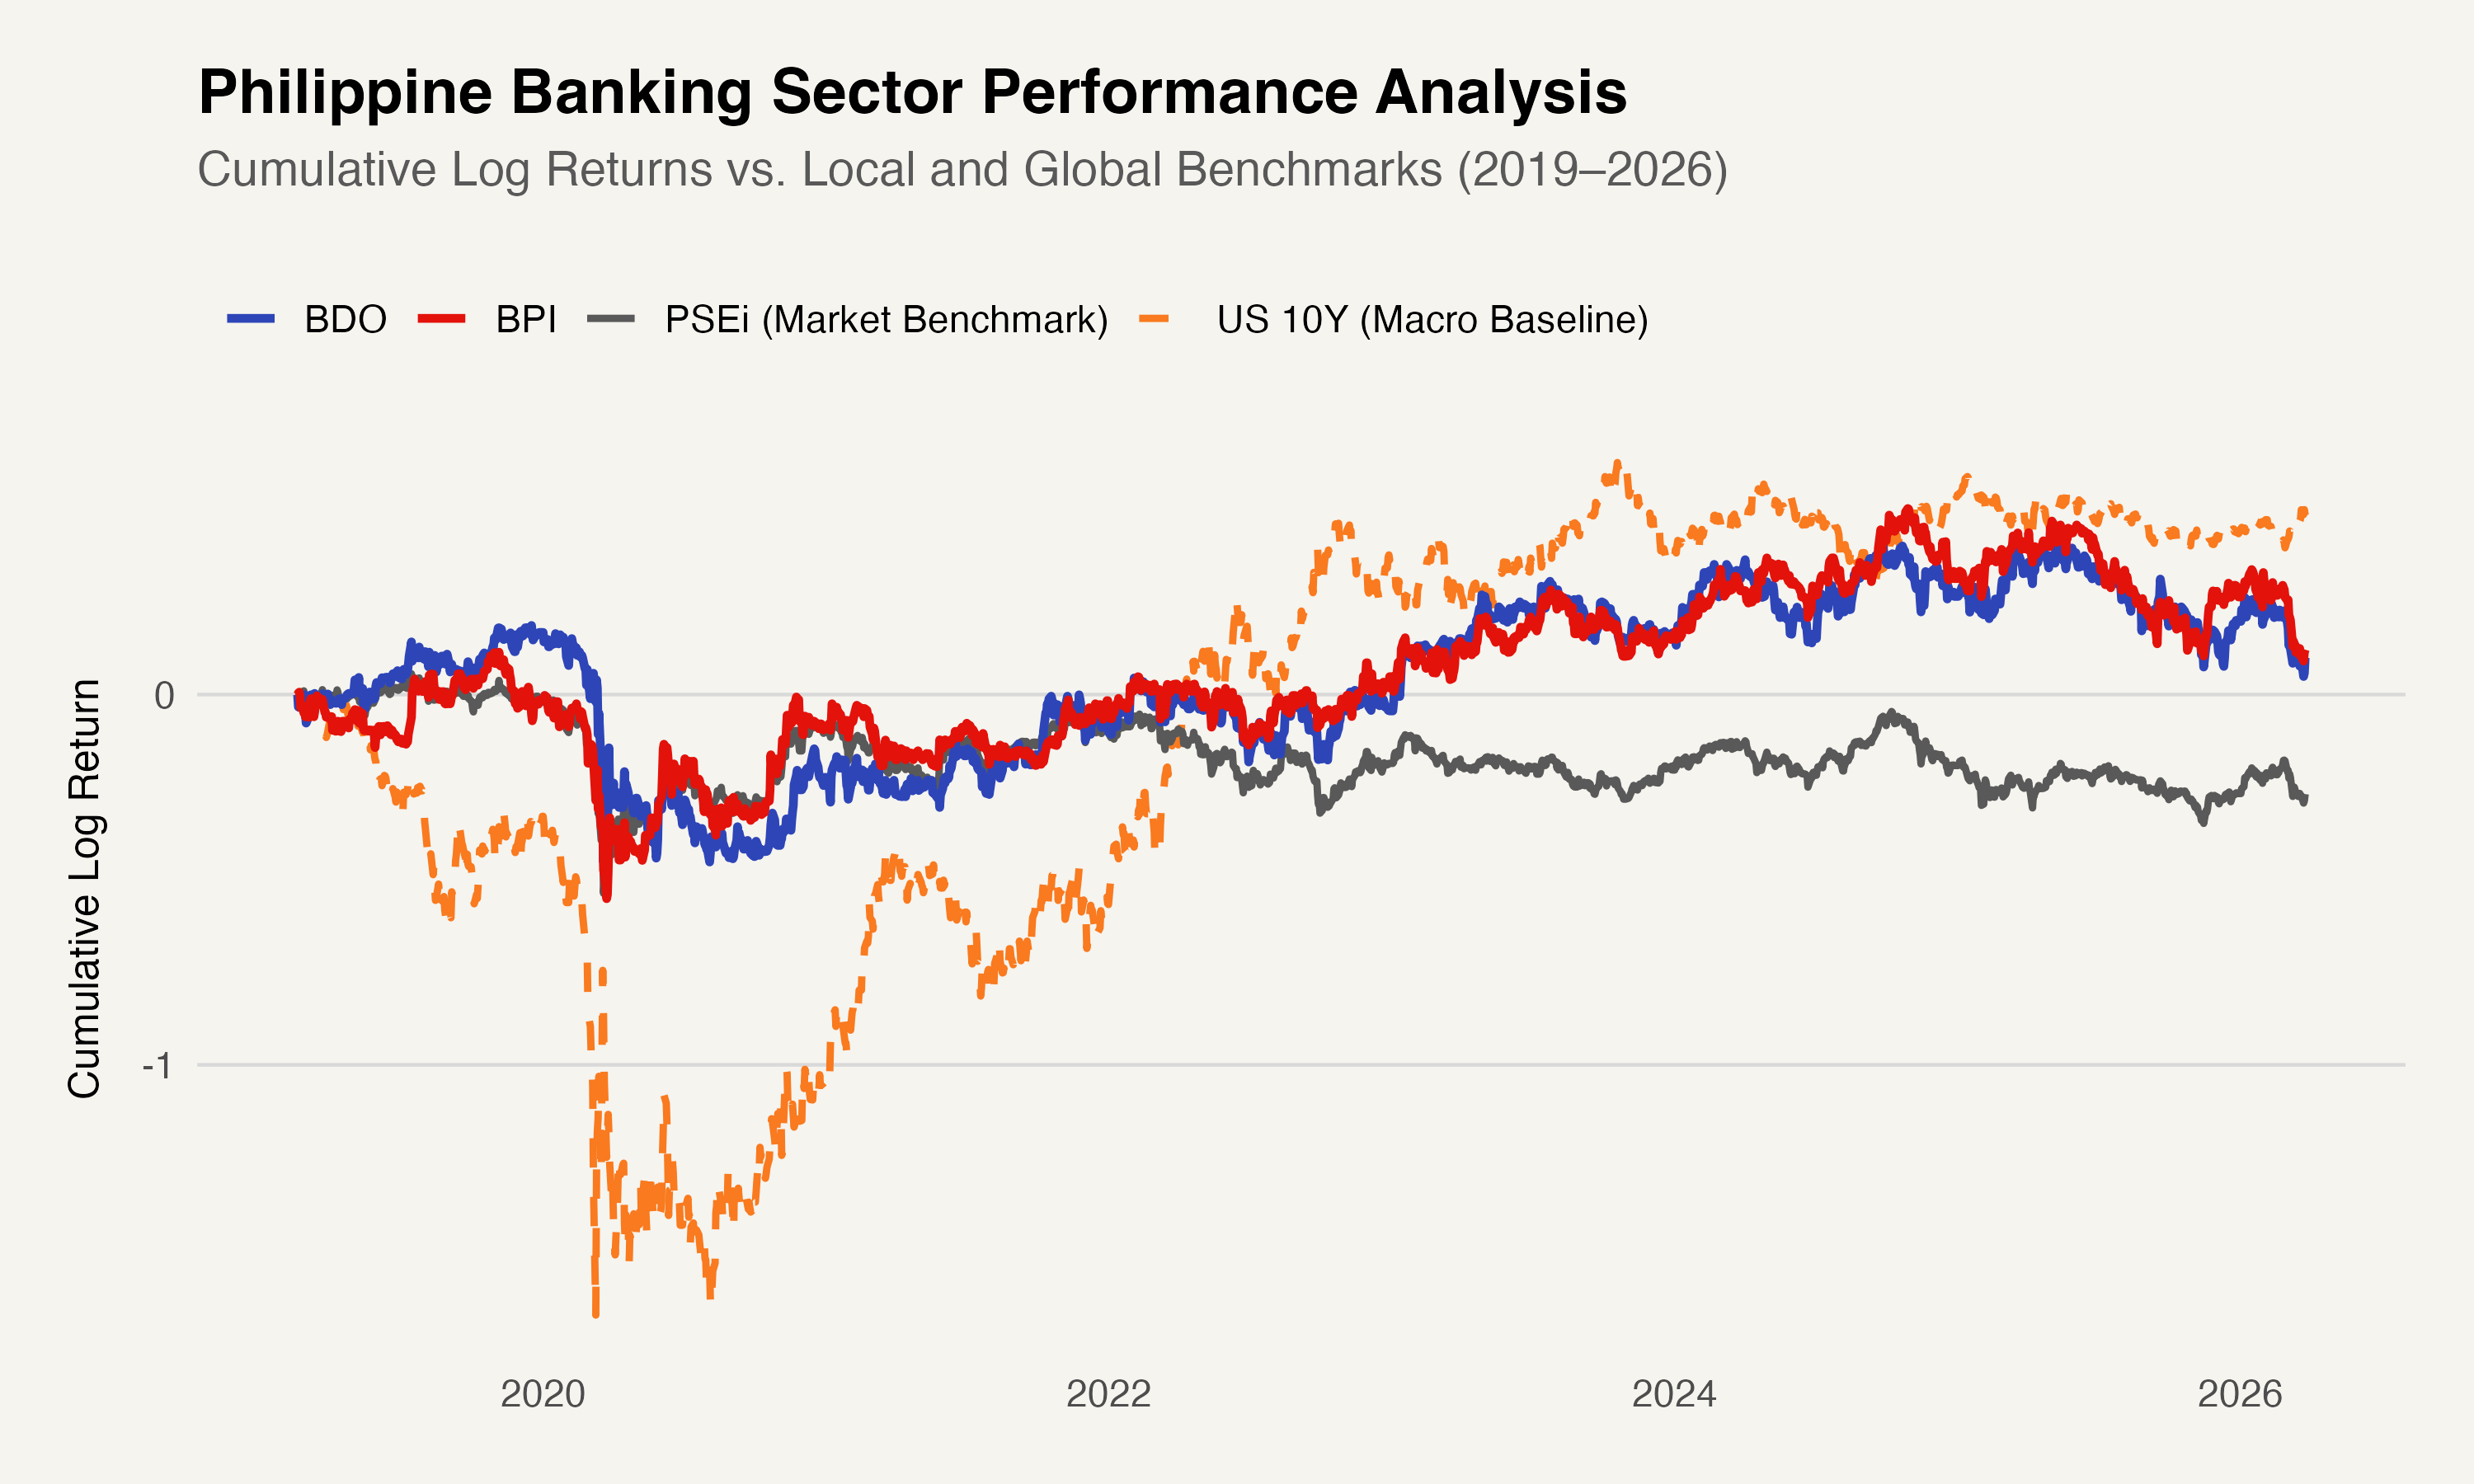
\includegraphics[width=0.8\textwidth]{figures/macro_correlation.png}
    \caption{Philippine Banking Sector Performance vs. Local and Global Benchmarks}
    \label{fig:macro_correlation}
    \textit{Note.} Normalized cumulative log returns (2019--2026). The divergence between domestic equity performance and rising U.S. yields illustrates the structural vulnerability of frontier market valuations to global liquidity tightening.
\end{figure}

\subsection{Feature Transformations and Regime Variable}

\subsubsection*{Feature Transformations}

Two engineered features are included to capture nonlinear and conditional relationships among the base indicators. An interaction term between the one-day lagged return and short-run realized volatility allows the models to detect whether momentum is predictive conditional on the prevailing risk environment:

\begin{equation}
    interact_t = r_{t-1} \times \sigma_{5,t}
\end{equation}

A squared short-run volatility term is included as a direct nonlinear transformation:

\begin{equation}
    vol^2_{5,t} = \left(\sigma_{5,t}\right)^2
\end{equation}

This term captures the convex relationship between extreme volatility states and subsequent return distributions, a pattern well-documented in empirical asset pricing \parencite{gu2020empirical}.

\subsubsection*{Regime Variable}

A data-driven binary indicator identifies high-volatility regimes without imposing calendar-based date restrictions:

\begin{equation}
    HiVol_t = \mathbf{1}\!\left[\,\sigma_{20,t} > 2\,\bar{\sigma}\,\right]
\end{equation}

where $\sigma_{20,t}$ is the 20-day rolling standard deviation of BPI log returns and $\bar{\sigma}$ is the historical mean of that series computed on the training set only, ensuring that the regime threshold is not contaminated by future information. A value of one flags periods in which near-term realized volatility is at least twice the long-run baseline---capturing episodes such as the March 2020 market dislocation and subsequent macroeconomic stress periods---without hardcoding specific dates.

\subsubsection*{Look-Ahead Bias Controls}

All features described in this section are constructed strictly from information available at or before time $t$. Moving-window operators reference only historical observations; no forward-looking quantities enter any predictor. The three target variables ($r_{t+1}$, $r_{t:t+3}$, $r_{t:t+5}$) are stored as separate lead-shifted columns and are never included among the predictors. The regime threshold $\bar{\sigma}$ is estimated on the training partition and applied to the test set without re-fitting, consistent with the strict time-series split described in Section~\ref{sec:methodology}.
\subsection{Descriptive Statistics}

Table~\ref{tab:descriptive_stats} reports summary statistics for the three target return series and a representative selection of constructed features, computed over the full sample from January 2, 2019 to April 1, 2026. Statistics include the sample mean, standard deviation, minimum, maximum, skewness, and excess kurtosis. As is typical for daily equity log returns, the target distributions are expected to exhibit near-zero means, substantial excess kurtosis relative to the normal distribution, and modest negative skewness reflecting asymmetric downside risk.

\begin{table}[!h]
\centering
\caption{\label{tab:descriptive_stats}Descriptive Statistics: Target Variables and Key Features (2019--2026)}
\centering
\resizebox{\ifdim\width>\linewidth\linewidth\else\width\fi}{!}{
\begin{tabular}[t]{lrrrrrr}
\toprule
Variable & Mean & SD & Min & Max & Skewness & Ex. Kurtosis\\
\midrule
$r_{t+1}$ (1-day return) & 0.0001 & 0.0194 & -0.1156 & 0.0940 & -0.2406 & 3.8844\\
$r_{t:t+3}$ (3-day cumulative) & 0.0001 & 0.0302 & -0.1923 & 0.2069 & 0.2001 & 4.2785\\
$r_{t:t+5}$ (5-day cumulative) & 0.0003 & 0.0372 & -0.2122 & 0.1857 & 0.0768 & 3.3420\\
$r_{t-1}$ (Lag 1 return) & 0.0001 & 0.0194 & -0.1156 & 0.0940 & -0.2405 & 3.8888\\
MA Ratio (5/20) & 1.0006 & 0.0306 & 0.8052 & 1.1471 & -0.4007 & 4.9262\\
RSI (14-day) & 50.5271 & 10.3353 & 20.7849 & 85.4483 & 0.1171 & 0.1846\\
$\sigma_5$ (5-day rolling vol) & 0.0174 & 0.0099 & 0.0018 & 0.0817 & 1.8427 & 5.6089\\
$r^{\text{PSEi}}_t$ (market return) & -0.0001 & 0.0124 & -0.1432 & 0.0717 & -1.3450 & 15.5454\\
$r^{FX}_t$ (USD/PHP return) & 0.0001 & 0.0034 & -0.0132 & 0.0162 & 0.1880 & 1.7010\\
$r^{US10Y}_t$ (US 10Y return) & 0.0003 & 0.0331 & -0.3470 & 0.4048 & 0.2756 & 31.1372\\
$HiVol_t$ (regime dummy) & 0.0178 & 0.1323 & 0.0000 & 1.0000 & 7.2859 & 51.1112\\
\bottomrule
\multicolumn{7}{l}{\rule{0pt}{1em}\textit{\textit{Note.}} Sample: January 2, 2019 to April 1, 2026 (1853 observations after initialization window removal). Ex. Kurtosis is excess kurtosis (0 for normal distribution). All returns are daily log returns.}\\
\end{tabular}}
\end{table}



% SECTION 4: METHODOLOGY
\section{Methodology}
\label{sec:methodology}

The predictive framework utilizes a hybrid approach. It integrates classical econometrics with non-linear machine learning architectures. The objective is to forecast multi-horizon log returns for the Philippine banking sector.

\subsection{Data Partitioning and Temporal Integrity}

Predicting financial time series requires a strict chronological split. Random shuffling is prohibited. It introduces look-ahead bias. The dataset spans from January 2, 2019, to April 1, 2026. This period comprises 1,853 daily observations. The first 80\% of the sample serves as the training set. The remaining 20\% is reserved for out-of-sample testing. This split ensures the models are evaluated on unseen market regimes. It simulates a real-world trading environment.

\subsection{Target Variable Construction}

The study estimates separate models for three distinct investment horizons. All targets are expressed as log returns. This transformation ensures stationarity.
\begin{enumerate}
    \item \textbf{1-day Return ($r_{t+1}$):} Defined as $\log(P_{t+1}/P_t)$. It represents short-term price discovery.
    \item \textbf{3-day Cumulative Return ($r_{t:t+3}$):} Defined as $\sum_{i=1}^{3} r_{t+i}$. It captures multi-day momentum.
    \item \textbf{5-day Cumulative Return ($r_{t:t+5}$):} Defined as $\sum_{i=1}^{5} r_{t+i}$. It reflects weekly trend persistence.
\end{enumerate}
All features are lagged at time $t$ or earlier. This eliminates data leakage.

\subsection{Model Specifications}

\subsubsection{Ordinary Least Squares (OLS) Benchmark}
The OLS model serves as the linear baseline. It assumes a constant relationship between features and returns. The specification follows $r_{t+k} = \alpha + \beta \mathbf{X}_t + \epsilon_t$. $\mathbf{X}_t$ represents the vector of technical and macro features. We utilize Newey-West standard errors. This adjustment accounts for heteroskedasticity and autocorrelation.

\subsubsection{Random Forest (RF)}
The RF model employs an ensemble of 500 decision trees. It uses bootstrap aggregation to reduce variance. The \texttt{ranger} engine implements this architecture. We tune the number of features per split (\textit{mtry}) and the minimum node size. This prevents the model from fitting to idiosyncratic market noise.

\subsubsection{Support Vector Machine (SVM)}
The SVM utilizes a Radial Basis Function (RBF) kernel. It maps features into a high-dimensional space to find non-linear hyperplanes. Feature standardization is mandatory. We scale all predictors to zero mean and unit variance. The scaling parameters are derived solely from the training set. We tune the cost parameter ($C$) and the kernel width ($\sigma$).

\subsubsection{Gradient Boosting (XGBoost)}
XGBoost implements a sequence of weak learners. Each tree corrects the residuals of its predecessor. It optimizes a regularized objective function. This prevents overfitting. We tune the learning rate, tree depth, and L1/L2 regularization terms. It is the most computationally efficient architecture in the suite.

\subsubsection{Artificial Neural Network (ANN)}
The ANN consists of a single-layer perceptron. It uses a decay parameter for regularization. The architecture identifies complex interactions through hidden neurons. We optimize the number of hidden units and the decay rate. This ensures the network does not memorize the training data.

\subsection{Validation and Hyperparameter Tuning}

Hyperparameter optimization utilizes a rolling origin cross-validation strategy. We employ the \texttt{rsample::rolling\_origin()} function. This method creates multiple training/validation slices. Each slice respects the temporal order. The model is trained on a window and tested on the immediate future. This process identifies the most robust parameters for non-stationary data.

\subsection{Evaluation Metrics}

We assess model performance through statistical and financial lenses. 
\begin{itemize}
    \item \textbf{Root Mean Squared Error (RMSE):} Measures the magnitude of prediction deviations.
    \item \textbf{Mean Absolute Error (MAE):} Provides a robust measure of average error.
    \item \textbf{R-squared ($R^2$):} Quantifies the proportion of variance explained.
    \item \textbf{Directional Accuracy (DA):} Calculates the frequency of correct sign predictions. This metric is the primary indicator of economic utility.
\end{itemize}
All models are compared against a naïve lagged-return benchmark.

% SECTION 5: RESULTS
\section{Results}
\label{sec:results}
% ASSIGNED TO: Person 3

\subsection{Visual Analytics}
% TODO

\subsection{Regression Results and Model Performance}
% TODO

% SECTION 6: DISCUSSION
\section{Discussion}
\label{sec:discussion}
% ASSIGNED TO: Person 4

\subsection{Model Comparison}
% TODO

\subsection{Horizon Analysis}
% TODO

\subsection{Feature Importance Interpretation}
% TODO

\subsection{Regime Effects}
% TODO

% SECTION 7: CONCLUSION AND RECOMMENDATIONS
\section{Conclusion}
\label{sec:conclusion}
% ASSIGNED TO: Keira

% REFERENCES
\printbibliography[title={References}]

\newpage
\appendix
\section{Technical Implementation Code} \label{sec:appendix_code}
{} The full source code for this analysis is available at:
\texttt{[INSERT GITHUB REPO URL HERE]}

All scripts are numbered sequentially (\texttt{01} through \texttt{06}) and
must be run in order. Data is pulled programmatically via the \texttt{tidyquant}
package. No manual data downloads are required.

\end{document}

document}
